\documentclass[11pt,twocolumn]{article}

\usepackage{fullpage}
\usepackage{subfigure,indentfirst}
% for url
\usepackage{hyperref}
% for underlined text
\usepackage[normalem]{ulem}
% for including pdf figures
\usepackage{graphicx}
\usepackage{xcolor}
\usepackage[utf8]{inputenc}
% for nice multiline equations
\usepackage{amsmath}

% my own versions: my_enumerate and my_itemize
\newenvironment{my_enumerate}{
  \begin{enumerate}
    \setlength{\itemsep}{1pt}
      \setlength{\parskip}{0pt}
\setlength{\parsep}{0pt}}{\end{enumerate}
}

\newenvironment{my_itemize}{
  \begin{itemize}
    \setlength{\itemsep}{1pt}
      \setlength{\parskip}{0pt}
\setlength{\parsep}{0pt}}{\end{itemize}
}

% start document
\begin{document}

\title{CS87 Project Report: Parallelized Computation of Superpixels}

\author{Rachel Diamond, Tai Warner, and Henry Han \\
Computer Science Department, Swarthmore College, Swarthmore, PA  19081}

\maketitle

%%%%%%%%%%%%%%%%%% ABSTRACT %%%%%%%%%%%%%%%%%%%%%
%%%%%%%%%%%%%%%%%%%%%%%%%%%%%%%%%%%%%%%%%%%%%%%%%
\begin{abstract}

%Briefly state the basic contents
%and conclusions of your paper: the problem you are solving, why the reader
%should care about this problem, your unique solution and/or implementation,
%and the main results and and contributions of your work.

%  For writing organization resources, see my
%  CS Research and Writing Guide:

%\noindent {\small \url{www.cs.swarthmore.edu/~newhall/thesisguide} } 

%And, off my help pages~\cite{newhall:help} are links to other resources 
%for technical writing, including a writing style guide and information
%about Unix tools for creating and editing figures.
Superpixelation involves grouping pixels in a way that captures some of the perceptual and intuitive meaning of an image. Superpixels are a useful tool for many computer vision problems including image segmentation and object recognition because superpixelation can be used as a preprocessing step that both reduces dimensionality and identifies more meaningful features. A good superpixel algorithm efficiently produces superpixels that respect object boundaries, are of approximately equal size, and are compact -- this means that superpixel edges fall along the edges of objects in the image, there is a roughly constant number of pixels per superpixel, and that each superpixel is relatively round. We implement a parallelized version of the simple linear iterative clustering (SLIC) algorithm for superpixelation with the goal of improving time efficiency and possibly scaling to larger image sizes. SLIC uses a $k$-means clustering approach which iteratively updates the assignment of pixels to superpixels based on the distance between the pixel and the superpixel centers. It is a good candidate algorithm for GPU parallelization because it has subparts that can computed independently by pixel or by superpixel. Although our results show that our parallelized implementation is 4-5 times slower than the sequential SLIC, we achieve nearly the same accuracy using metrics calculated using UC Berkeley's Segmentation Benchmarks - especially as the number of superpixels increase. 
%Our results show that we were able to improve the runtime for computation of superpixels by \textcolor{red}{XXX\%} relative to the sequential implementation. However, the data transfer off the GPU is a current bottleneck which leaves the parallel implementation \textcolor{red}{XXX\%} slower than the sequential version.

\end{abstract}

%%%%%%%%%%%%%%%%%% INTRO %%%%%%%%%%%%%%%%%%%%%%%%
%%%%%%%%%%%%%%%%%%%%%%%%%%%%%%%%%%%%%%%%%%%%%%%%%
\section {Introduction} 

%The introduction is the big picture of your work: what, why, and how. It
%includes a definition of the problem you are solving, a high-level description
%of your solution including any novel techniques and results you provide, and a
%summary of the main results of your paper. In addition, motivates the problem
%you are solving (why should a reader find your work important), and describes
%your contribution to the area (this may not be applicable to your project).
%The first paragraph of the introduction should contain all of this information
%in a very high-level. Subsequent paragraphs should discuss in more detail the
%problem you are solving, your solution, and your results and conclusions.

Superpixels are an approach to image segmentation in which the pixels are grouped together in a way that graphically approximates the information contained in the image. For example, regions of the same color should be grouped together, and edges between two objects in a picture should correspond to a boundary between two superpixels. 

\begin{center}
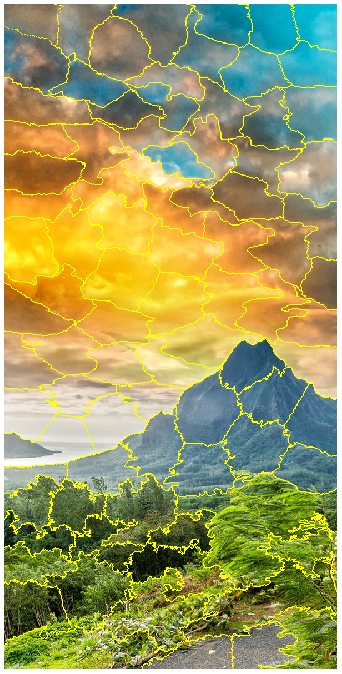
\includegraphics[width = 0.6\linewidth]{mountain100.png} \\
\end{center}
\textit{Figure 1.} An example of SLIC segmenting an image into superpixels and superimposing the boundaries (shown in yellow) over the image. \\

Superpixels can be useful in computer vision as a step toward object recognition; seeing objects as collections of constituents is an intuitive goal for machines. A superpixel could also provide a viewer with a better idea of what an image is about since it contains information about the shape of the region and the variation in color within the region, as opposed to a single colored pixel, which would give a viewer no idea what the image contains. Superpixelation can even be used to create compressed representations of images if the color variation within a superpixel is discarded in favor of just the superpixel's shape and average color. 

One example application where superpixelation served as an important preprocessing step is in Lucchi et. al's (2010) work \cite{medical} to identify mitochondria in an electron microscope (EM) image of neural tissue. This is a particularly difficult object localization and recognition problem because, as can be seen in Figure 2(a), the edges of mitochondria look very similar to other features in the EM image, mitochondria are irregularly shaped, there are many structures in a single image, and textures clutter the background. Lucchi et. al's were able to improve on previous results by introducing a new algorithm that starts by segmenting the image into superpixels. Then a vector of shape and color features were calculated for each superpixel. These features and the training data shown in Figure 2(c) are then used to train an Support Vector Machine (SVM), which is predictive model that classifies whether each superpixel is mitochondial boundary. The final steps map back from superpixels to pixels and apply smoothing to get a final segmentation.

\newpage
\begin{center}
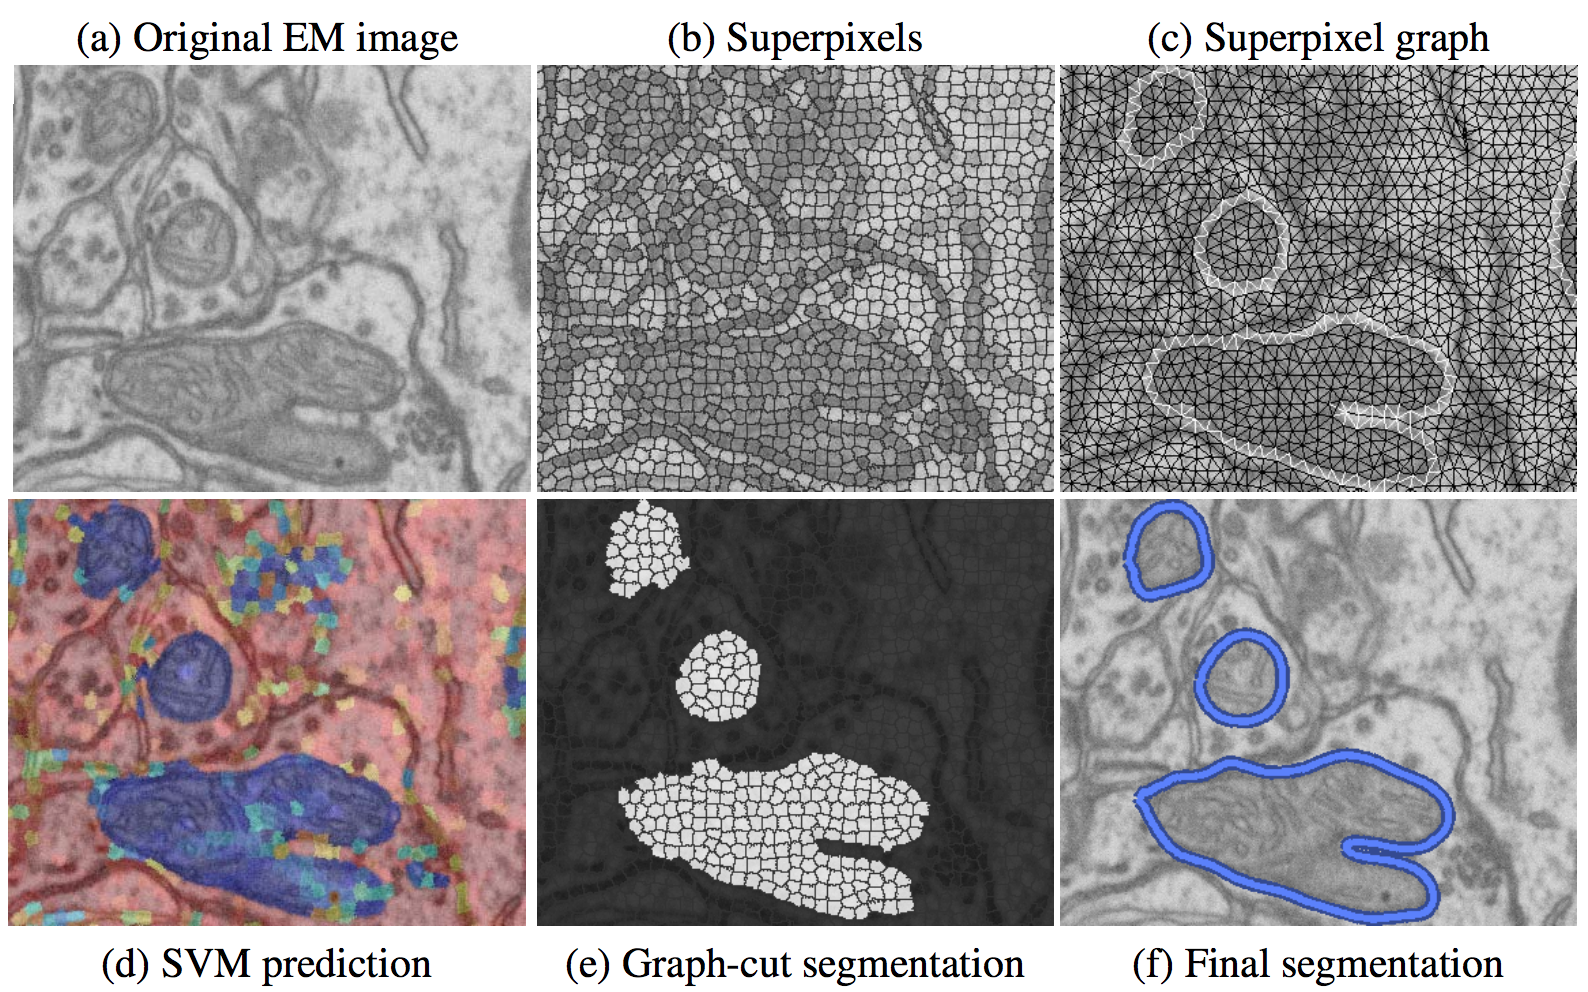
\includegraphics[width = \linewidth]{application.png} \\
\end{center}
\textit{Figure 2.} \footnote{Figure from Lucchi et. al (2010) \cite{medical}.} Basic steps of an object localization algorithm that uses SLIC to identify mitochondria in an image of neural tissue. (a) Original image. (b) Superpixel segmentation. (c) Graph defined over superpixels. White edges indicate pairs of superpixels used to train an SVM
that predicts mitochondrial boundaries. (d) SVM prediction where blue indicates a probable mitochondrion.
(e) Graph cut segmentation. (f) Final results after automated post-processing. \\
%\hline\noalign\\

We use Achanta et al's (2010) simple linear iterative clustering algorithm, SLIC, as a baseline to implement our own version parallelized on the GPU. SLIC is based on the classic machine learning algorithm $k$-means clustering. Section \ref{kmeans} has a detailed explanation of $k$-means, but at a high level, we begin with $k$ pixels at even intervals designated as the centroids. We then run (usually) ten iterations where pixels are assigned to centroids and then centroids are adjusted to have the average color and location of their assigned pixels. This causes centroids to settle into $k$ local optima, generally representing the centers of $k$ representative constituents of the image. The simplicity of the algorithm allows it to perform with surprising speed given its accuracy. However, substantially sized images --- for example, landscapes shot in high resolution --- can take up to a minute due to the repetitive nature of the algorithm multiplied over millions of data points.

Our extension to SLIC is parallelism on the GPU. For this, our system consists of eight Intel i7 cores and a NVIDIA Quadro P5000. We parallelize over the pixels in the image; while the GPU can assign each thread its own pixel up to about ten trillion pixels, we hope to quickly reach a speedup of a few thousand, when all the cores of the GPU are exploited, which should happen even with an image as small as 50x50 pixels.

At the end of this paper, we discuss our experimental design and results. We present the results of tests that access quality of performance of parallel and sequential implementations and the runtime efficiency of each. We use a metric of boundary recall to assess quality, where the intuition is that high boundary recall means that our superpixelation captures most of the contrast between objects in the image. We also measure total time taken for the program to run and compare these results between sequential and parallel runs of SLIC.

%%%%%%%%%%%%%%%%%% RELATED WORK %%%%%%%%%%%%%%%%%
%%%%%%%%%%%%%%%%%%%%%%%%%%%%%%%%%%%%%%%%%%%%%%%%%
\section {Related Work}\label{relwork}

% This is an essential part of a research paper; discussing related work is a
% good way to put your work in context with other similar work, and to provide a
% way for you to compare/ contrast your work to other's work.  You should use
% feedback on the annotated bibliography from your project proposal to structure
% this section; it should be written as a re-write of your annotated bibliography
% in a single Related Work section.

%\textcolor{red}{Talk a little about other paradigms of superpixel algorithms but don't go in detail about how they work}

Achanta et. al (2010, 2012) \cite{slic}\cite{slic2012} introduced the SLIC algorithm, a new technique for solving the problem of image superpixelation. While older algorithms existed that use graph-based or gradient ascent methods, SLIC is built on a $k$-means clustering approach. This is conceptually much simpler, because it intuitively clusters in terms of the color and position of pixels -- two pixels that are a similar color but far away are not likely to be part of the same object, just as two nearby pixels of starkly different color are probably part of different objects. It is also a simpler algorithm computationally, and takes orders of magnitude less time than some other superpixel algorithms. 

Some SLIC extensions have already been explored and implemented. For example, gSLIC is a parallel implementation of SLIC that uses CUDA to run on the GPU \cite{gslic}. gSLIC achieved an impressive 19 times speedup when compared to SLIC for the largest image size that they tested (1280 x 960 pixels). ASLIC, or Adaptive SLIC, is an implementation of SLIC that doesn't require the programmer to tune any hyperparameters \cite{slic2012}.

Our parallelized version of SLIC differs from gSLIC in that we primarily used Python and PyCuda (A Python wrapper to use Nvidia's CUDA parallel computation API in C/C++)  to parallelize th e kernels, whereas gSLIC is written entirely in C++. 

Prior to SLIC, there were other approaches to image superpixelation that used graph-based (GS04, NC05) or gradient-ascent-based (WS91, MS02) algorithms. In graph based algorithms, each pixel becomes a node in a graph, and the edge weights are set to be proportional to the similarity between pixels. In gradient ascent based algorithms, the algorithm uses gradient ascent methods to refine clusters (after an initial rough clustering) and obtain better segmentation \cite{slic}.  As shown in Figure 3, in terms of metrics for image superpixelation, i.e. speed, boundary recall, etc., SLIC outperforms all of the other algorithms \cite{slic}.\\

\begin{center}
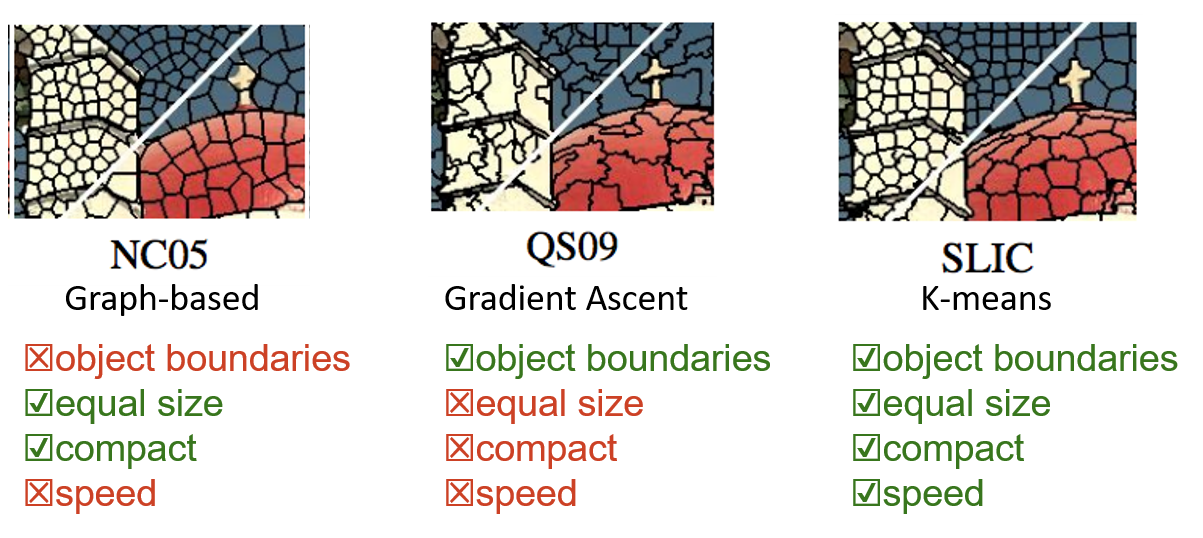
\includegraphics[width = \linewidth]{slic_comp.png} \\
\end{center}
\textit{Figure 3.}\footnote{Segmented images by Achanta et. al (2012) \cite{slic2012}.}This figure shows that neither NC05, a graph-based algorithm, nor QS09, a gradient-ascent-based algorithm, can outperform SLIC in all four of the following metrics regarding the superpixels created by the algorithms: object boundaries, equal size, compactness, and runtime. \\

%%%%%%%%%%%%%%%%%% OUR SOLN %%%%%%%%%%%%%%%%%%%%%
%%%%%%%%%%%%%%%%%%%%%%%%%%%%%%%%%%%%%%%%%%%%%%%%%
\section {Our Solution}\label{soln}
%Details of the problem you are solving Details of your solution and the
%project's implementation Even though you may have spent an enormous amount of
%time writing code, this should not include a listing of any code you wrote.
%Only if your project is about developing an algorithm or a new language, may
%code examples be appropriate here.  Discussion of how your solution solves the
%problem.

The SLIC algorithm implements local $k$-means clustering to group pixels together based on their color similarity and proximity. Instead of comparing pixels in the canonical RGB color space, our implementation of SLIC assumes an image in CIELAB color space which represents color in terms of dimensions referred to as $l$, $a$, and $b$ respectively. The CIELAB color space is generally regarded as perceptually uniform for small color distances and is intended to more closely match how humans perceive color \cite{slic}. Our implementation combines color information and location on the image for each pixel, effectively mapping each pixel in a 2-dimensional image into 5-dimensional $labxy$ space. Our implementation extends to higher dimensional space to support segmentation of 3-dimensional images in 6-dimensional $labxyz$ which allows superpixelation of video. Because we didn't get to experimenting in 6-dimensional $labxyz$ space with videos, $z$ is 1 in all our experiments. 

%%%%%%%%%%%%%%%%%%%%%%%%%%%%%%%%%%%%%%%%%%%%%%%%%
\subsection{k-Means}\label{kmeans}
The $k$-means clustering algorithm is a machine learning algorithm that aims to iteratively classify $n$ observations into $k$ clusters by assigning each observation to the cluster that is nearest to it by some given distance measure. As shown in Figure 4, cluster centers can be initialized randomly or based on a preset arrangement. The algorithm will then run iteratively for a fixed number of repetitions or until the number of observations reassigned to a new cluster from one step to the next falls below a set threshold. Each iteration has two steps:  expectation and maximization.

During the expectation step, the distance of each observation to each cluster center is calculated and the observation is assigned to the cluster that is the closest to it based on a given distance measure (usually Eucleadian distance). Next, during the maximization step, the cluster centers are re-calculated based on the average of the new member observations.

\begin{center}
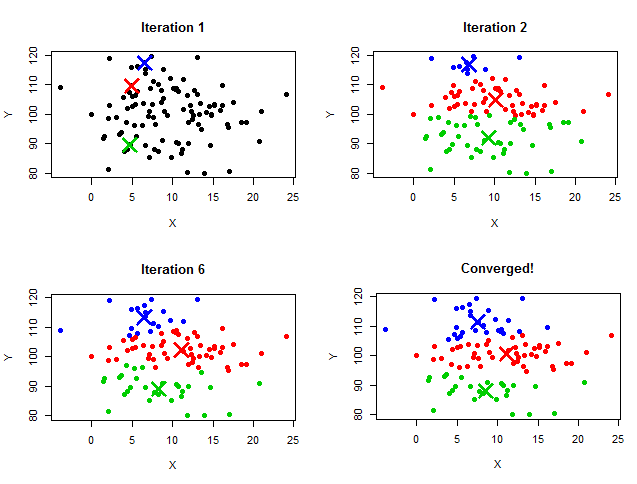
\includegraphics[width = \linewidth]{kmeans_example_cropped.png} \\ 
\end{center}
\textit{Figure 4.} \footnote{Taken from \url{http://www.learnbymarketing.com/methods/k-means-clustering/} } In Iteration 1, cluster centers are initialized and represented as colorful crosses. The observations are associated with the closest clusters in iteration 2. By iteration 6, the cluster centers have clearly shifted around as they are recalculated in the maximization step. In the last plot, we can see that the algorithm has converged and every observation is now associated with its closest cluster. \\

In our implementation of SLIC, each pixel in the image is an observation that the algorithm clusters into one of $k$ superpixels. We initialize cluster centers, which we call centroids, as the centers of an evenly spaced rectangular grid over the image. Then we run ten iterations of the expectation-maximization steps. Achanta et. al found that ten iterations is usually sufficient to minimize the residual error after reassigning centroids \cite{slic}, so we default to ten iterations as well. Also in accordance with Achanta et. al's method, we implement a local (as opposed to global) $k$-means algorithm. This means that during the expectation step, instead of calculating the distance from each pixel to each centroid, we only calculate the distance from each pixel to each centroid within a $2S \times 2S$ window, where $S = \sqrt{\frac{n}{k}}$, $n$ is the number of pixels, and $k$ is the number of centroids, or superpixels. We can restrict the search area for each pixel because we expect similar pixels that should be in the same superpixel to be nearby one another. 

Implementing a local $k$-means instead of searching globally and limiting the algorithm to ten iterations improves the runtime from $O(kni)$ to $O(n)$, where $k$ is the number of centroids, $n$ is the number of pixels, and $i$ is the number of iterations for the $k$-means algorithm. This modification drastically reduces the number of calculations in the expectation step - instead of calculating the distance from each pixel to all centroids, which is $O(kn)$, local $k$-means only requires a constant number of calculations from each pixel to each centroid within a $2S \times 2S$ window. This makes the expectation step just $O(n)$. 

\subsection{Distance Measure}
Because we are working in 6-dimensional $labxyz$ space, we use a special distance measure $D_{s}$, defined as follows:

\begin{equation}
d_{lab} = \sqrt{(l_{k} - l_{i})^2+(a_{k}-a_{i})^2+(b_{k}-b_{i})^2} \\
\end{equation}
\begin{equation}
d_{xyz} = \sqrt{(x_{k}-x_{i})^2+(y_{k} - y_{i})^2 + (z_{k}-z_{i})^2} \\
\end{equation}
\begin{equation}
D_{s} = d_{lab} + \frac{m}{S}d_{xyz}
\end{equation}

Here, $D_{s}$ is the sum of the $lab$ distance and the $xyz$ plane distance normalized by the grid interval $S$, and $m$ is the compactness factor. This hyperparameter $m$ allows us to control the compactness of a superpixel by emphasizing spacial proximity during the normalization of the spatial distances. \cite{slic}. Figure 5 shows the effect of varying $m$ on an image.

\begin{center}
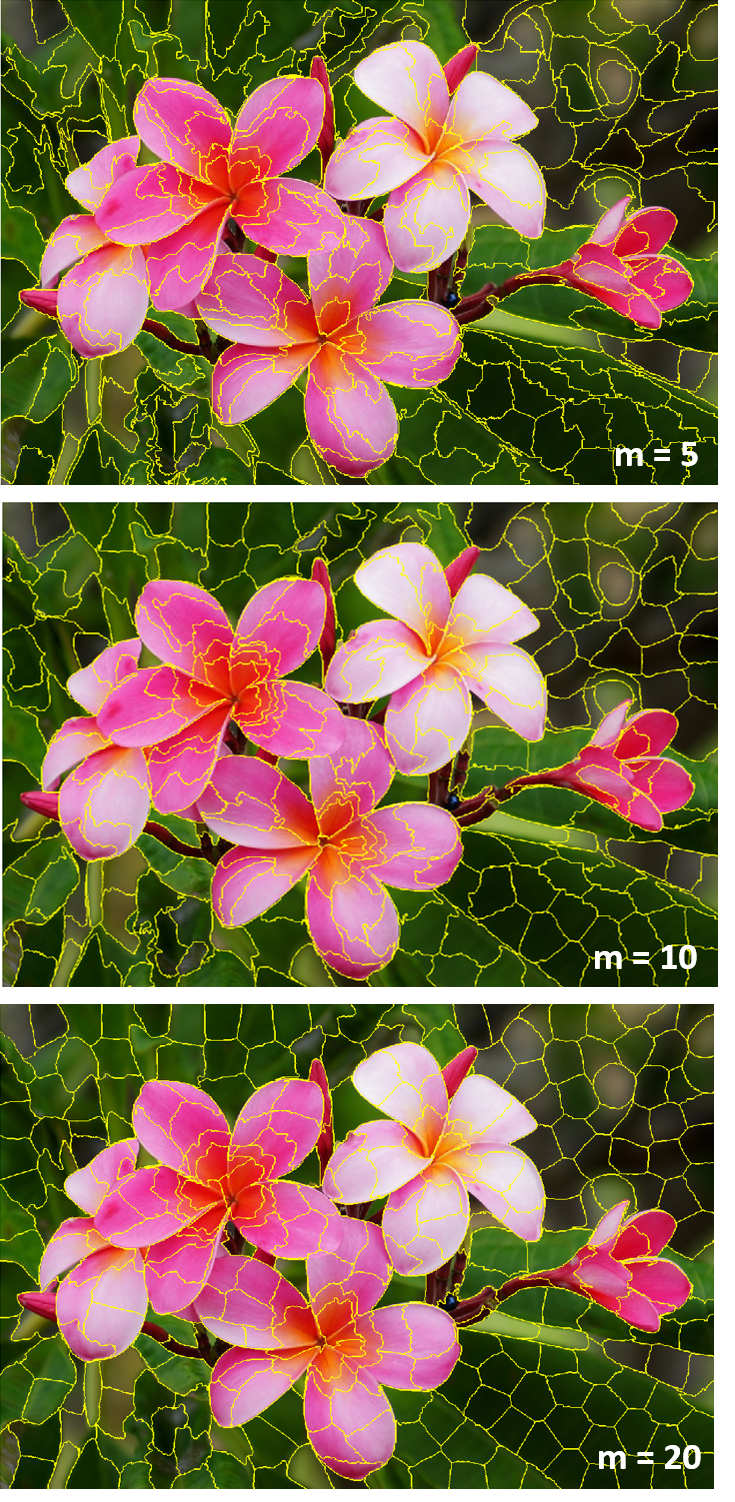
\includegraphics[width = \linewidth]{flowers.png} \\ 
\end{center}

\textit{Figure 5.} This figure shows the impact of the compactness factor $m$. As m increases, spatial proximity is emphasized and the superpixels become more compact. This results in smoother and rounder superpixels. 

%%%%%%%%%%%%%%%%%%%%%%%%%%%%%%%%%%%%%%%%%%%%%%%%%
\subsection{CUDA Parallelism}

%Our solution parallelizes by pixel. 

For a more modular, powerful, and conceptually easier coding environment, we break up the pipeline of SLIC. We designate three main parts which are parallelized in separate CUDA kernels: the initial assignment of pixels throughout the image to centroids, the assignment of pixels to the closest centroid, and the recalculation of the centroid locations. We also draw from specific knowledge about CUDA architecture in some of the choices we make about the design of the parallelism. In order to quickly reach maximum parallelism, we parallelize over pixels and assign one thread per pixel. With this design choice, it makes the most sense to store the data for the algorithm in three large arrays representing the color values of each of $n$ pixels, the $k$ average coordinate values of each centroid, and the mapping of each of $n$ pixels to its assigned centroid. This allows us a parallelism factor up to $n$ for the first assignments (since it just consists of populating the assignments array), and update assignments (since it involves each pixel assessing candidate centroids for the new closest). The recomputing of the centroids reaches a parallelism factor of $k$, since there are $k$ centroids.

The first assignments function simply uses as many threads as there are pixels in the image, and uses the thread ID to map each thread to a unique pixel. Then, it calculates the $xyz$ coordinates of the pixel and uses this to calculate the identity of the nearest centroid. (This designation is easy to figure out beforehand, but the function to update assignments which will be described later involves searching for the nearest centroid.) This function does not need to return anything to the CPU before calling the next function.

Once the first assignments are made, we enter a loop which is the expectation-maximization part of this algorithm. Importantly, this loop cannot be parallelized because each round relies on the state resulting from the last round. This loop consists of recomputing centroids (the expectation step), and adjusting pixels' assignments to them (the maximization step). Recomputing centroids is parallelized over $k$ threads on the GPU, and each thread takes the average value in 6-dimensional $labxyz$ space of its (on average) $\frac{k}{n}$ member pixels. These measurements are embarrassingly parallel, but there is not an easy way to further parallelize them on the GPU, so each thread loops through every member. By the end of this function, the array of centroids has been updated.

Finally, we update the assignments. Again, this is parallelized over all $n$ pixels in the image. However, now each thread must do a certain number of checks to make sure that a new centroid has not become closer than the old one. For this, we make the assumption that the final centroid that a pixel ends up associated with will be one of its closest initially. The ``close" region is defined by three centroids in each dimension. For 2-dimensional images, this means we look at a local region that includes nine centroids, and calculate the distance to each. Most of the time, when this function finishes, we go back to recomputing the centroids, but after the final iteration, we copy the memory that has been manipulated by the GPU back to the CPU in order to post-process and visualize it.

%%%%%%%%%%%%%%%%%% RESULTS %%%%%%%%%%%%%%%%%%%%%%
%%%%%%%%%%%%%%%%%%%%%%%%%%%%%%%%%%%%%%%%%%%%%%%%%
\section {Results}\label{results}
%Experimental Results demonstrating/proving your solution Explain the tests you
%performed (and why) Explain how you gathered the data and details of how your
%experiments were run (any system/environment set up) Present your results
%Choose quality over quantity; the reader will not be impressed with pages and
%pages of graphs and tables, instead s/he wants to be convinced that your
%results show something interesting and that your experiments support your
%conclusions.  Discuss your results!  Explain/interpret your results (possibly
%compare your results to related work). Do not just present data and leave it up
%to the reader to infer what the data show and why they are interesting. 
Our experiments are run on the computer \textit{anise} at Swarthmore College which has eight Intel i7 cores and a NVIDIA Quadro P5000 graphics card.

%%%%%%%%%%%%%%%%%%%%%%%%%%%%%%%%%%%%%%%%%%%%%%%%%
\subsection{Timing Metric}
A central goal of implementing a parallelized version of SLIC is to decrease the time that it takes to produce a superpixel segmentation. This is especially desirable if SLIC is being used as a preprocessing step for a computer vision task like object recognition, because the overall algorithm can only be as efficient as its component parts.

To test the efficiency of our parallelized implementation of SLIC we used timing code to determine runtime on a single square image scaled to five different edge sizes: 128, 256, 512, 1024, and 2048px. We used the same image scaled so that the complexity of the image itself would have minimal effect on the timing. We ran the sequential SLIC implementation on the same set of five images. We also varied the number of superpixels $k$ in order to see how this affected runtime. We expect increasing image size to lead to longer runtime because many more computations must be performed. We also expect that increasing the number of superpixels will have little effect on sequential runtime, but it will improve performance of the parallel algorithm because the recompute centroids function is parallelized in terms of the number of superpixels. 

We ran five repetitions of each set of hyperparameters and averaged the results to account for potential variation in background programs that could affect the timing results.

%%%%%%%%%%%%%%%%%%%%%%%%%%%%%%%%%%%%%%%%%%%%%%%%%
\subsection{Timing Results}

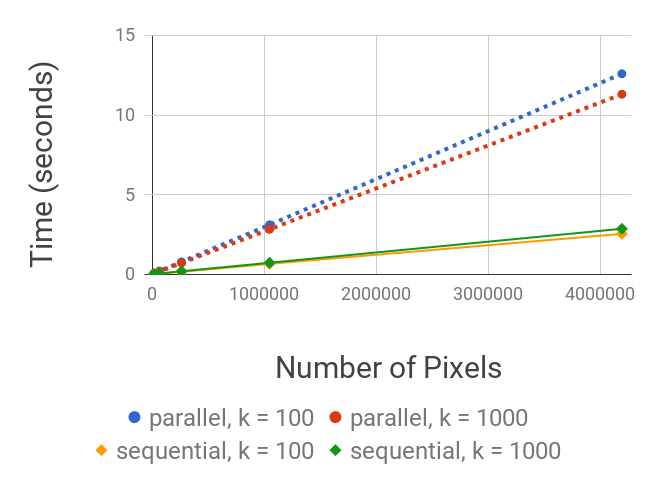
\includegraphics[width = \linewidth]{timing_results.png} \\

\textit{Figure 6}. Timing results for the parallel (solid lines) and sequential (dotted lines) implementations of SLIC as image size and number of superpixels is varied. \\

As shown in Figure 6, both the parallel and sequential versions of SLIC had runtimes that scaled linearly in the number of pixels, regardless of the number of superpixels. The sequential version of SLIC was 3.7 times faster for $k=1000$ and 4.9 times faster for $k=100$ when averaged across image sizes. This was unexpected given that the purpose of parallelism is to reduce runtime. We did a more detailed breakdown of how time is spent within the algorithm to determine if the relatively long execution time for the parallel implementation was due to copying memory between the CPU and the GPU. However, we determined that the majority of the time was in fact spent within the kernel calls for recomputing superpixel centroid locations and updating the assignment of pixels to superpixels.

As expected, the number of superpixels did not significantly affect the runtime of the sequential algorithm. With 1000 rather than 100 superpixels, the parallel algorithm was 11.1\% faster when averaged across image sizes.

%%%%%%%%%%%%%%%%%%%%%%%%%%%%%%%%%%%%%%%%%%%%%%%%%
\subsection{The Boundary Recall Metric}
Boundary recall is a metric that tells us the percentage of the actual object boundaries in the image that our algorithm correctly labels as a segmentation boundary. Using the metrics true negative (TN), false negative (FN), false positive (FP), and true positive (TP), boundary recall is defined as 

\begin{equation}
boundary\ recall = \frac{TP}{FN + TP}
\end{equation}

This means that if our algorithm has a boundary recall of $0.60$ for a given image, then $60\%$ of the boundaries in the image are also located where there is a superpixel boundary identified by our algorithm. 

To test our algorithm's boundary recall, we used David Stutz's benchmark code written as an extension to the \href{https://www2.eecs.berkeley.edu/Research/Projects/CS/vision/grouping/resources.html}{Berkeley Segmentation Benchmark} that is meant to provide performance metrics for contour detection and image segmentation \cite{benchmark}. 

Figure 7 shows both the inputs to the benchmark code and the output from our SLIC algorithm. To calculate boundary recall, we provided the benchmark code with three images: the original image, the ``correct" or ground truth segmentation of the image, and a contour map of the superpixel segmentation that our algorithm generated. The superpixel segmentation and the image with superpixel boundaries superimposed onto it are both outputs of our SLIC algorithm. 

\begin{center}
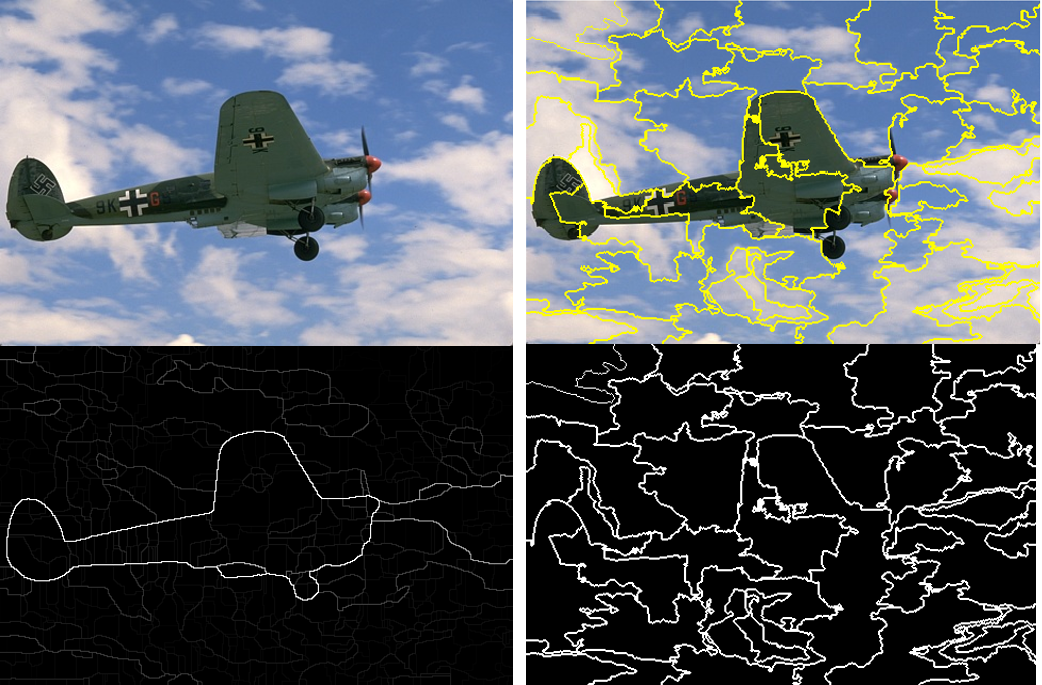
\includegraphics[width = \linewidth]{grouped.png}
\end{center}
\textit{Figure 7}. Clockwise from upper left: the original picture, the original picture with superpixel boundaries from our algorithm superimposed onto it (yellow lines), superpixel boundaries our algorithm determined, and the ``correct" segmentation from by the Berkeley Segmentation Benchmark \cite{benchmark} dataset. \\

%%%%%%%%%%%%%%%%%%%%%%%%%%%%%%%%%%%%%%%%%%%%%%%%%
\subsection{Boundary Recall Results}
We ran experiments with David Stutz's extension on Berkeley Segmentation Benchmark by varying the number of superpixels $k$, the compactness factor $m$, for the sequential and parallel implementations of SLIC.

The boundary recall results presented in Figure 8 largely make sense. Boundary recall was expected to increase as the number of superpixels increase simply because an increase in the number of superpixels will increase the total number of boundaries. This increases the likelihood that the ``correct" ground truth boundaries will also be segmentation boundaries. This was shown to be true for both the parallel and sequential implementations.  

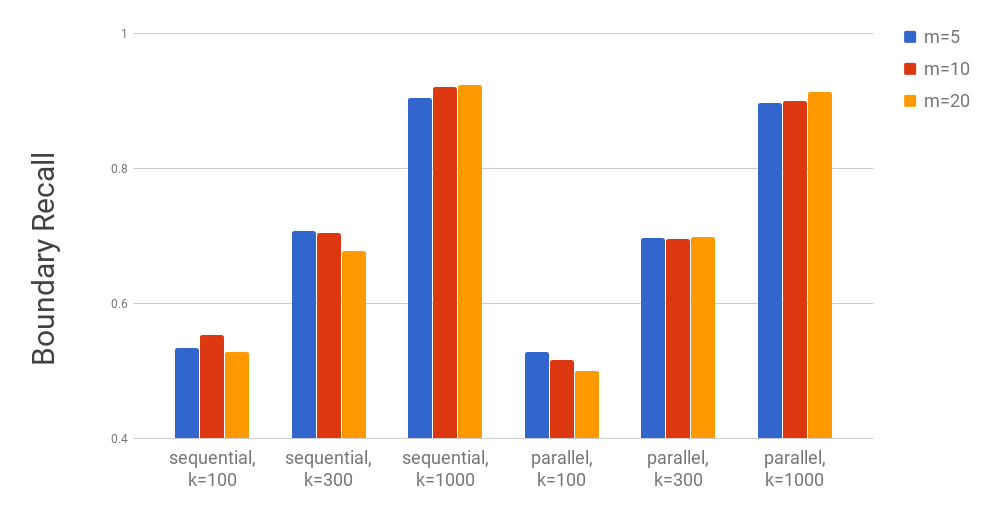
\includegraphics[width = \linewidth]{boundary_recall.png} \\
\textit{Figure 8}. As shown in the chart, boundary recall to increases significantly as the number of superpixels increases. The sequential version of SLIC has slightly higher recall than our parallel implementation. A low compactness factor appeared to do better for lower values of $k$, and a high compactness factor appeared to do better for higher values of $k$. \\

When $m$ is small, SLIC appears to do better when $k$ is small as well for both the parallel and sequential implementations. This is also expected because with less superpixels and less enforced spatial compactness, the algorithms are more likely to capture the segmentation boundaries in the ground truth with jagged and rougher edges in each superpixel. As $m$ gets bigger, the algorithms do better when $k$ is bigger. This is because as the images become heavily segmented it is naturally able to capture the segmentation boundaries in the ground truth. With a larger value of $m$, spatial proximity is emphasized and the superpixel boundaries will be smoother and more naturally capture boundaries in the image. 

In theory, we expect the sequential and parallel algorithms to produce the same superpixels and thus produce the same boundary recall measures. However, because our parallelization of the code differs slightly from the sequential version in order to effectively parallelize the code, the superpixels differ and thus the boundary recall measures do as well. This is most notable when both $m$ and $k$ are small. 

All in all, our parallel version of SLIC performs nearly as well as the sequential version of SLIC, especially as the number of superpixels and the value of the compactness factor increases.

%%%%%%%%%%%%%%%%%% CONCLUSTIONS %%%%%%%%%%%%%%%%%
%%%%%%%%%%%%%%%%%%%%%%%%%%%%%%%%%%%%%%%%%%%%%%%%%
\section{Conclusions and Future Work}\label{conc} 
%Conclusions and Future Directions for your work Conclude with the main ideas
%and results of your work. Discuss ways in which your project could be
%extended...'s next? what are the interesting problems and questions that
%resulted from your work? \textcolor{red}{Need to fill out}

%%%%%%%%%%%%%%%%%%%%%%%%%%%%%%%%%%%%%%%%%%%%%%%%%
\subsection{Conclusions}
We expected to achieve a significant reduction in runtime by parallelizing the SLIC algorithm for superpixels. However, our parallelized version of SLIC was about 4-5 times slower than the sequential version. It is not clear why our parallel implementation was drastically slower, but we suspect that our parallel kernels had synchronization and concurrency problems as we tried to hack them together. We think this problem was compounded by the fact that we implemented the algorithm in Python and parallelized with PyCuda. We chose to implement SLIC in Python because we thought it would be easier, but the high level coding style actually became an obstacle when we were parallelizing the code. Now that we really understand the concepts behind the algorithm, it would be smoother to implement SLIC in C or C++. We also originally suspected that the slower runtime was due to copying memory back and forth between the CPU and the GPU. However, we determined that the majority of the time was actually spent within the kernel calls for recomputing the superpixel centroid locations and updating the assignment of pixels to superpixels. On the other hand, even though our algorithm didn't perform better in terms of speed, it achieved nearly the same boundary recall accuracy, especially as the number of superpixels and the value of the compactness factor increased.
%%%%%%%%%%%%%%%%%%%%%%%%%%%%%%%%%%%%%%%%%%%%%%%%%
\subsection{Future Work}
SLIC has been implemented with a number of extensions since its conception. GPU parallelism is one, dubbed gSLIC, as well as ASLIC, a zero-parameter version of SLIC which adaptively assesses the visual activity in a region and lowers compactness in highly textured areas in order to more accurately represent the irregular constituents. This provides a simple next step building off of our work presented here --- a GPU parallelism of SLICO would likely require little more than a change to the objective function within the kernel to update assignments.

There are also a few potentially interesting niches of research to be filled with SLIC-based applications. While our work presented in this paper focuses on 2-dimensional images which results in 5-dimensional $k$-means, a 6-dimensional version could allow for object recognition and tracking through time. An example would be an application of SLIC over a movie. For this, all frames in the movie would be consolidated into a 3-dimensional block of images, like stacking thousands of sheets of paper together into a block. Now there is a sixth axis, $t$, for time. In this representation, a ball being thrown across the screen would be represented by a diagonal worm shape --- in the early frames, the ball is on one side but as its position in $t$ increases, its $xy$ position changes, too. Ideally for this version of the problem, the algorithm would try to find the 3-dimensional supervoxels that make up the ball's path. The distance function would have to be changed, and we suspect that there should be less compactness along $t$ as along $x$ and $y$, since $t$ isn't spatial in the same way as the latter two.

SLIC could be used for general purpose data compression. Like the boom of GPGPU computing, which conceived of regular problems as matrices in order to take advantage of the GPU's propensity for projecting planes, regular data could be conceived of as an image, and compressed using SLIC. SLIC is a convenient algorithm for compression because the user can choose $k$; the closer $k$ is to $n$, the less compressed the output is. By this token, a dataset could be compressed, while still hopefully preserving the general distribution and outline of the original data. We suspect that a SLIC-based compression would be less accurate than some other well-known machine learning techniques for dimensionality reduction given the scale of the compression, although Lucchi et al (2010) have shown that more meaningful new dimensions can be extrapolated from the output given by SLIC.\cite{medical}

%%%%%%%%%%%%%%%%%% META %%%%%%%%%%%%%%%%%%%%%%%%%
%%%%%%%%%%%%%%%%%%%%%%%%%%%%%%%%%%%%%%%%%%%%%%%%%
\section{Meta-discussion}\label{meta}

%A brief meta-discussion of your project Include two paragraphs in this section:
%Discussion of what you found to be the most difficult and least difficult parts
%of your project.  In what ways did your implementation vary from your proposal
%and why?  
We originally intended to parallelize SLIC in the first week, implement SLICO (adaptive SLIC that self-tunes $m$) by week 2, experiment with 6-dimensional supervoxels, and extend gSLIC and SLICO to create gSLICO - a parallelized version of SLIC that adaptively tunes $m$. We think we fell short of our goals for a number of reasons, but bad documentation and starting code was likely the biggest. 

Initially, we intended to write our implementation in CUDA C++. This quickly became confusing and hard to read, and we decided it would be simpler and more modular in Python. We used PyCUDA, an appropriation of CUDA to a Python environment, to help connect with the GPU. However, while the documentation is not bad, it leaves something to be desired in terms of thorough explanation, return values, and especially error messages. We experienced a hangup for over a week due to an error that was impossible to find a helpful discussion of on the internet. In addition, there is no GDB for a Python environment, so this type of low-level error tracing was especially difficult. While this turbulence between low- and high-level created some tension in our work flow, there were a number of benefits that the high-level aspect of this project provided: namely, image interpretability. In presenting our project, we time and again were able to show listeners our generated images while we were talking to them about the particular algorithm, and this multimedia approach allowed people who were less interested in the math to grasp the function of the algorithm intuitively, while also being able to connect the math to varying behavior between different runs of the program.



%At the end of your paper is a Reference section. You must cite each paper that
%you have referenced...your work is related to some prior work.

% The References section is auto generated by specifying the .bib file
% containing bibtex entries, and the style I want to use (plain)
% compiling with latex, bibtex, latex, latex, will populate this
% section with all references from the .bib file that I cite in this paper
% and will set the citations in the prose to the numbered entry here
\bibliography{finalreport}
\bibliographystyle{plain}

%%%%%%%%%%%%%%%%%% APPENDICES %%%%%%%%%%%%%%%%%%%
%%%%%%%%%%%%%%%%%%%%%%%%%%%%%%%%%%%%%%%%%%%%%%%%%
% force a page break
%\newpage 
%\onecolumn
%\section{Appendices}\label{appx} 

%You may optionally add appendices to your report.  They do not count towards
%page total.  Appendicies are for expanding on details or results that are
%beyond inclusion in the main part of paper.  It could be where you have code
%snippets that illustrate some of details of what you discuss, but it is not a
%venue for a dump of all the code you wrote, which has no place in research
%paper.  

%\textcolor{red}{may put full parallel pseudocode here}

\end{document}

